\chapter{%
深層学習による配管6D姿勢推定}

従来のアイソメ図取得にはLIDARセンサーにより3次元点群を取得し図面を作成していたが、
センサーが高価であるというデメリットを抱えていた。そのため、本研究ではLIDARセンサーよりも
比較的安価なRGB-Dカメラを用いてデータセット収集から深層学習やアイソメ図作成までの流れを紹介する。
第2.1節ではRGB-Dカメラを用いた深層学習による配管6D姿勢推定の手順を述べる。
第2.2節では物体認識のネットワーク設計を詳しく説明する。


\section{配管6D姿勢推定方法}
RGB-Dカメラを用いた深層学習による配管のアイソメ図作成の手順はデータ収集、物体検出、6D姿勢推定、アイソメ図作成の4つに分けられる。
図2.1にそのプロセスの流れを示す。

\begin{figure}[htbt]
	\centering
	 \includegraphics[height=65mm]{system.eps}
	 \caption{RGB-Dカメラを用いた深層学習によるアイソメ図作成方法}
	 \label{fig:f2}
\end{figure}

まず、RGB-Dカメラを用いてRGB画像とDepth画像を取得する。これらの画像を使用して物体検出ネットワークより複数の配管検出を行う。
次に、物体検出で認識された配管の姿勢を推定する。その際に、データセットとしてRGB画像から3次元復元ツールであるColmapを使用して
点群データを取得する。このColmapはStructure from Motion(SfM)という技術で異なる視点からの写真を使用して3次元形状を復元する
写真解析ソフトウェアである。Colmapから得られた点群データをもとに姿勢推定問題に取り組む。
最後に姿勢推定された結果を用いてアイソメ図を作成するが、図面には配管の距離情報を示す必要がある。
そのため、Depth画像を用いることで認識された配管のスケールを算出することができる。以上のステップを踏むことでRGB-Dカメラから
アイソメ図を作成することができる。

\section{配管の特徴を活かしたアイソメ図作成方法}
配管の形状には配管固有の特徴が存在する。図2.2に一部配管の例を示す。
配管は両端部分を除くと直線であるという特徴があるため、両端の曲管又はT字管がどの方向を向いているのかを認識できればその間を直線で結ぶことで
アイソメ図を作成することができる。そのため、本研究においては配管全体を認識するのではなく、画像内の曲管及びT字管を検出し姿勢を推定する。
それに加え、両端の曲管又はT字管間の距離をDepth画像を用いて算出することで図面を作成することができる。

\begin{figure}[htbt]
	\centering
	 \includegraphics[height=55mm]{pipe.eps}
	 \caption{配管の検出例}
	 \label{fig:f2}
\end{figure}

\section{ネットワーク構造}

\subsection{全体構成}
本研究では曲管及び、T字管の物体検出と6D姿勢推定を深層学習を用いて推定する。その全体構成を図2.3に示す。
物体検出ネットワークではRXD Layer用いたRXDネットワークを提案する。RGB画像とDepth画像をRXD Layerに挿入することで
それぞれの画像から抽出された特徴を結合し認識精度向上を図ることができる。また、姿勢推定ネットワークではGen6Dモデルを使用する。
Gen6Dは複数物体の検出ができないが、RXDネットワークから認識された複数の配管のピクセル座標とスケールをGen6DのSelectorに
それぞれ渡すことでRefinerを通して最終的に画像内の全ての曲管及びT字管の姿勢を求めることが可能になる。

\subsection{RXDネットワーク}
物体検出に使用するRXDネットワークについて紹介する。RXDネットワークの構成を図2.4に示す。RGBガメラから取得されたRGB画像とDepth画像を
それぞれConvolutional setに挿入することで特徴を抽出することができる。深層学習は基本的に層を深くすることで認識精度が向上するため、RXDネットワークでは複数回畳み込み層を使用している。
また、畳み込みの際にはBatch Normalization(BN)、ReLU、Max Pooling(MP)を各層に取り入れている。Batch Normalizationは各バッチのデータを使用し正規化を行う。
その結果、出力が適度に分散され、勾配消失などの問題が起こりにくくなり、学習が適切に進む。特に深めのネットワークを使用したときに、数カ所に挟むことで効果を得る。
次にMax PoolingとはCNNで用いられる基本的なプーリング層である。最大値プーリングではカーネル内の最大値のみを残すプーリング処理である。これらの層を複数利用することで
特徴をより濃くすることができる。

\begin{figure}[htbt]
	\centering
	 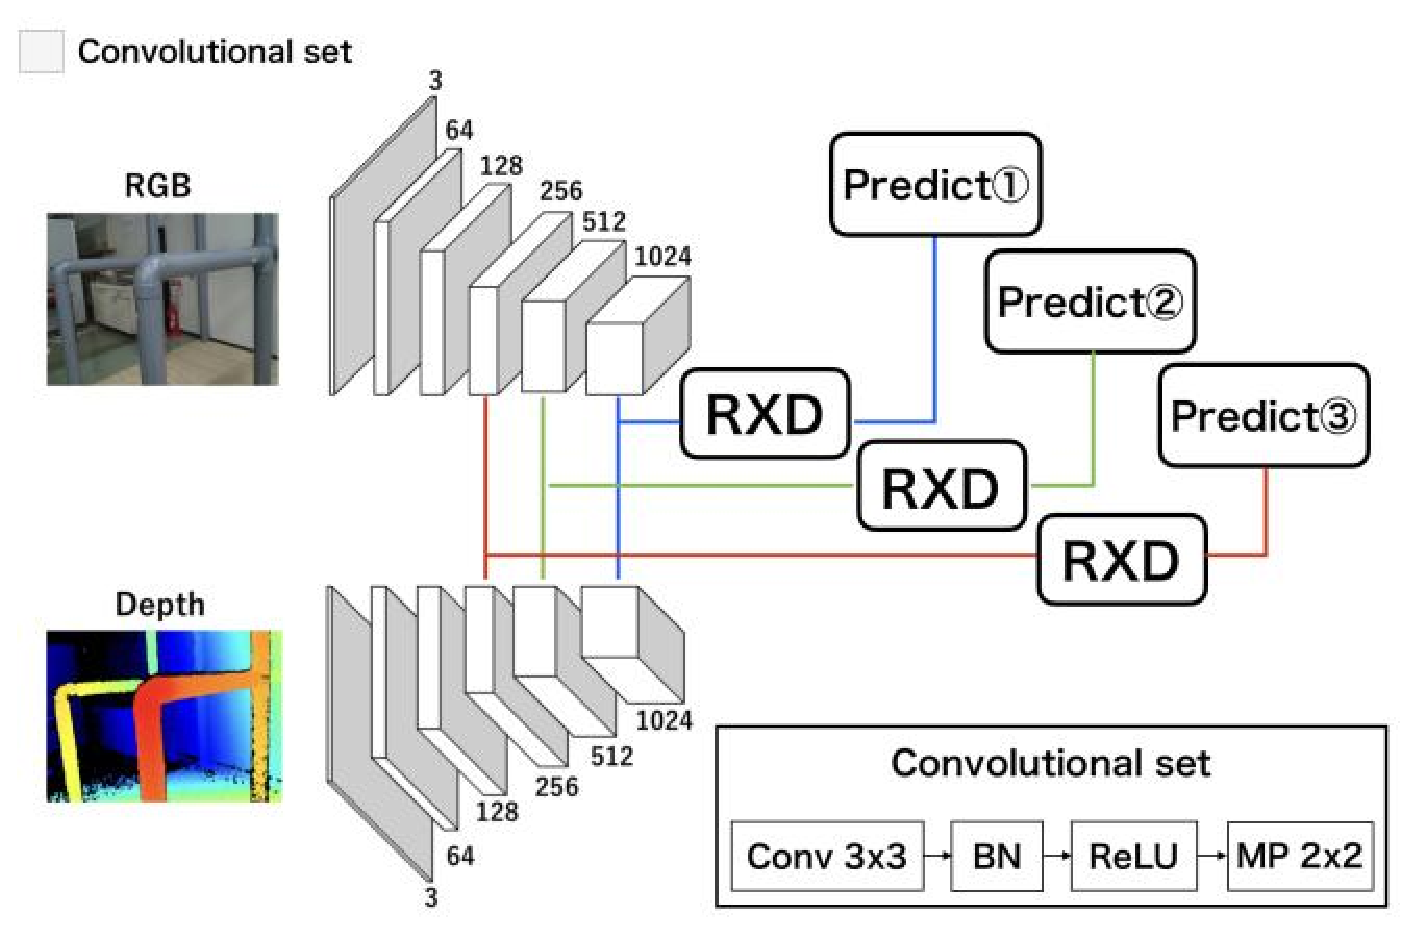
\includegraphics[height=95mm]{RXDnet.eps}
	 \caption{RXDネットワーク構造図}
	 \label{fig:f2}
\end{figure}

RXD層の内部構成を図2.5に示す。RXD層の中身ではRGB画像とDepth画像がRXDネットワークで畳み込まれたデータを結合する役割を担っている。
まず、RGB画像とDepth画像をそれぞれ畳み込み特徴マップを取り出す。それらのデータをConcatenate関数を用いて連結させる。
次に、結合されたデータを畳み込んだあとはSigmoid関数という活性化関数を使用する。
\begin{figure}[htbt]
	\centering
	 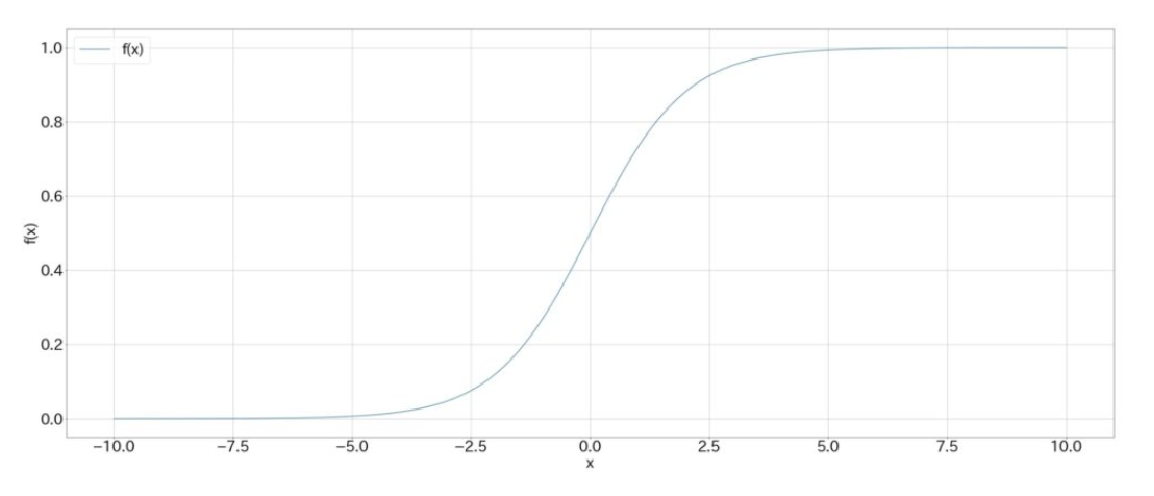
\includegraphics[height=65mm]{sig.eps}
	 \caption{Sigmoid関数のグラフ}
	 \label{fig:f2}
\end{figure}
通常の活性化関数にはReLU関数が使用され、入力が0以下の時は0を、0より大きい時はその値を出力する関数である。Sigmoid関数はReLU関数とは違い、
入力値xの値に依らず、0~1の数値に変換して出力する。
次に、Sigmoid関数によって出力された値をそれぞれもとのRXDネットワークから入力されたデータと乗算する。このステップによりRGB画像とDepth画像の
相関を利用し特徴マップの表現力を強化することができる。これによって得られたそれぞれの値をConcatenate関数を用いることで結合し、
2度の畳み込み層を経ることで出力結果が求められる。


\begin{figure}[htbt]
	\centering
	 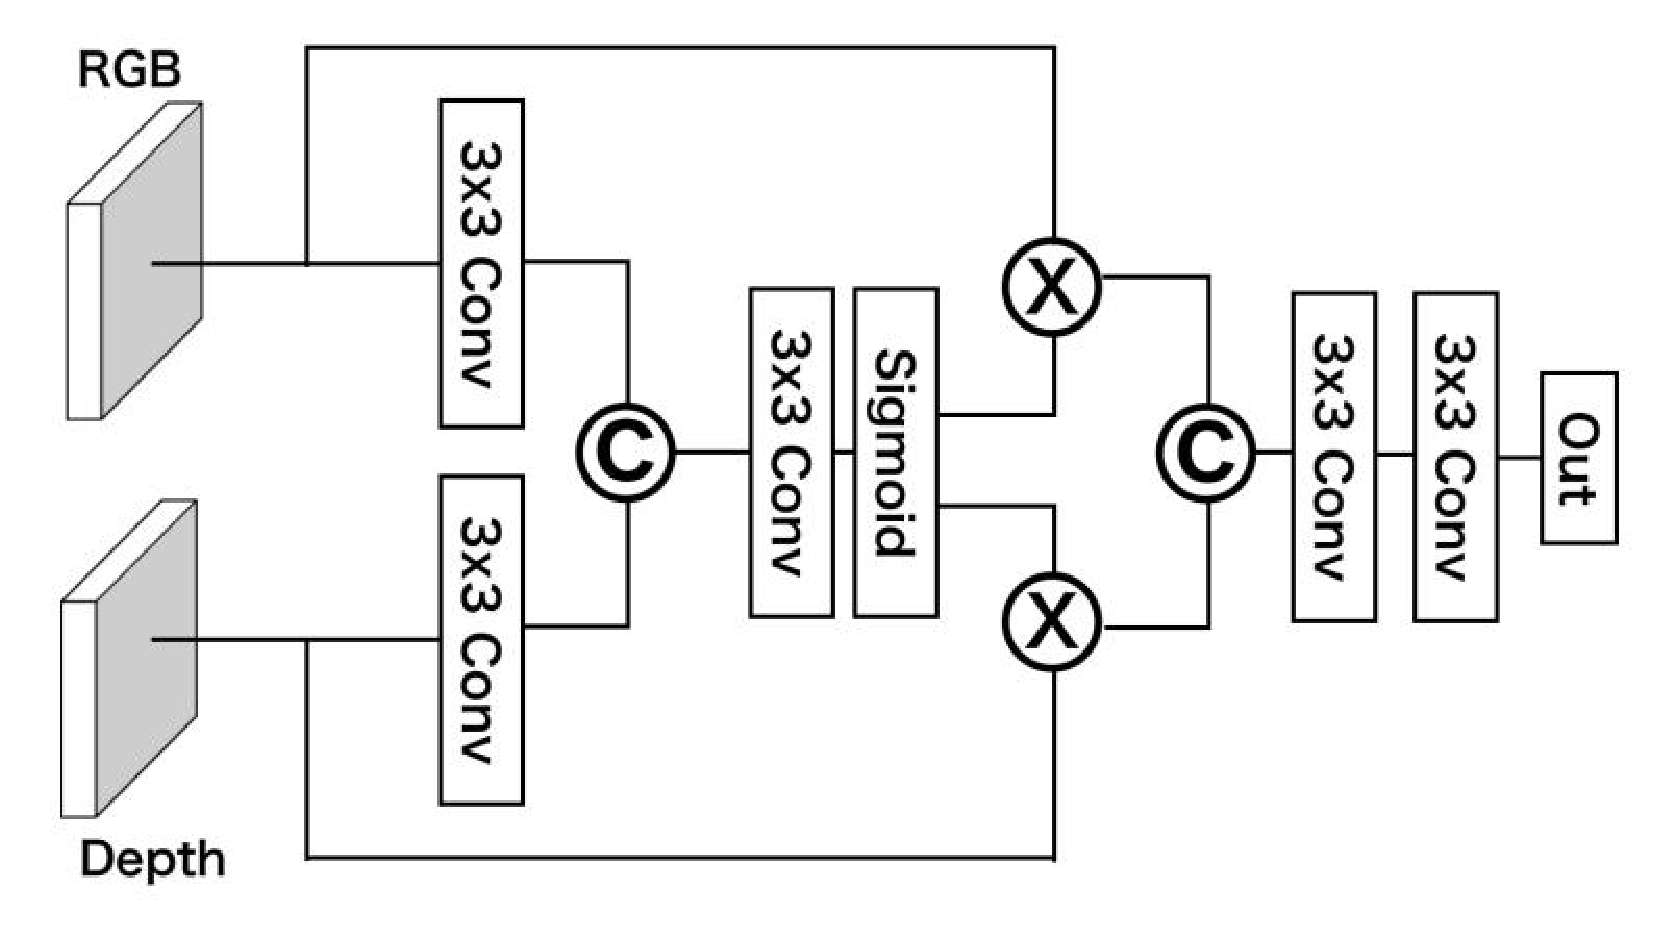
\includegraphics[height=85mm]{RXD.eps}
	 \caption{RXDネットワーク構造図}
	 \label{fig:f2}
\end{figure}



